\chapter{Experiments}

In this chapter we present our results and compare them to existing approaches.

\section{Datasets and metrics}

Dummy text.

\subsection{Datasets}

To get the Wikipedia pages, we use the dump from \emph{01 October 2012} that
has only the latest revision for each article \todo{Footnote for where to get
it}. The dump version we use should not impact the results considerably. We
happen to use the 2012 version just because was easily available at the time.
For this Wikipedia version we extract articles corresponding to a category (or
multiple categories recursively) recursively -- we parse the category graph
downwards starting from the given \emph{root} category. After extracting the
articles we keep only non-stub, human-written articles and we exclude all meta
pages. For more information about the extraction process see
\todo{coverage.WikiToPlainText section}.

We tested our approach on the following recursively extracted categories:
\begin{description}
  \item[Classical composers] Contains \(7246\) articles representing all
  classical music composers -- this is our biggest category apart from using all
  Wikipedia;
  \item[Game \acl{AI}] Contains \(471\) articles about the use
  of \ac{AI} in games (for example, chess, go, video games);
  \item[Machine learning] Contains \(735\) articles about the machine learning
  field;
  \item[Vectors] Contains \(341\) articles about mathematical vectors -- this
  our most abstract category;
\end{description}
and merges of them:
\begin{description}
  \item[Last 3] Contains the \(1547\) articles of the last three categories
  described above (Game \ac{AI}, Machine learning, Vectors);
  \item[All 4] Contains the \(8793\) articles of all above categories
  (Composers, Game \ac{AI}, Machine learning, Vectors).
\end{description}
For the final results we use the \textbf{2012 Wikipedia} which has a total of
\(1.3\) million \todo{double check this number} non-stub, human-written
articles (excluding meta pages). Out of space considerations we only present
the results we get on the whole Wikipedia.

In addition to the Wikipedia subset, we use the \emph{\acf{NIPS}} dataset --
contains \(1955\) papers -- and the \emph{\acf{ACL}} dataset -- contains
\(18041\) papers -- to test our baseline implementations against their authors
\cite{sipos2012temporal}.

\subsection{Metrics}

We have looked to find metrics suitable to our task of finding the most
important, valuable Wikipedia articles, but we could not find a reliable method
that also fits well to our use case.
Some of the possible metrics are:
\begin{description}
  \item[Number of inlinks] This metric is similar to the use of \emph{number of
  citations} presented in \cite{sipos2012temporal}, but extended to web pages.
  While it does not have the same limitations as citations, it is hard to
  guarantee its validity \todo{citation needed}.
  \item[PageRank] A common way to extend the use of just inlinks which solves a
  lot of the problems with inlinks.
  \todo{citation needed}.
  \item[Condensed Wikipedia] Count the number of selected documents that appear
  in a condensed Wikipedia version used in education or in emph{Wikispeedia}
  \todo{citation needed}.
\end{description}

For the purposes of this thesis we use \emph{number of inlinks} as we view
Wikipedia as a non-competitive environment (different from the game between
search engines and malevolent web masters).

\subsection{Interpreting the results}

For the experimental part, we use each submodular function to select the
\emph{top 40} articles out of all Wikipedia.

\subsubsection{Graphs}
To compare the different functions we score the \(40\) selected articles by a
given function with all the other functions and plot the scores as bar graph.
A function value of \(1\) means that the given set performs just as good as the
set selected by that function.
In other words, if the set selected by \emph{graph coverage} has a score of
\(0.77\) with \emph{word coverage} it signifies that it performs \(77\%\) as
good as the set selected by maximising \emph{word coverage}.
The \emph{\(X\) axis} represents the name of the functions used to compute that
score and the names refer to the following submodular functions:
\begin{description}
  \item[base] word coverage;
  \item[influence] document influence;
  \item[graph] graph coverage;
  \item[base+lsh-buckets] word coverage linearly combined with LSH buckets;
\end{description}
and a series of functions from Definition~\ref{def:coverage-of-word} from
Section~\vref{sec:word-coverage++}, where we vary the definition of \(\phi(d,
w)\):
\begin{description}
  \item[revcount] tf-idf \(\cdot\) number-of-revisions;
  \item[revcount-revvolume] tf-idf \(\cdot\) number-of-revisions \(\cdot\)
  revisions-volume;
  \item[inlinks-revvolume] tf-idf \(\cdot\) number-of-inlinks \(\cdot\)
  revisions-volume;
  \item[inlinks-revcount] tf-idf \(\cdot\) number-of-inlinks \(\cdot\)
  number-of-revisions;
  \item[inlinks] tf-idf \(\cdot\) number-of-inlinks;
  \item[revvolume] tf-idf \(\cdot\) revisions-volume;
  \item[inlinks-revcount-revvolume] tf-idf \(\cdot\) number-of-inlinks
  \(\cdot\) number-of-revisions\(\cdot\) revisions-volume.
\end{description}

\subsubsection{Tables}
In the tables we show the \emph{top 20} articles among the selected \(40\).
The columns have the following meaning, in order from left to right:
\begin{enumerate}
  \item article rank;
  \item article name;
  \item number of inlinks.
\end{enumerate}

\section{Baselines}

We consider three baselines:
\begin{enumerate}
  \item random;
  \item word coverage;
  \item document influence.
\end{enumerate}

\subsection{Random}

To generate the random sets we sample without replacement \(40\) articles from
among the \(1.3\) \emph{million} human-written Wikipedia articles. We repeat
the process \(10\) times and report the \emph{mean} along with one
standard-deviation bars. \todo{Add the stdev bars.}

\begin{figure}
  \centering
  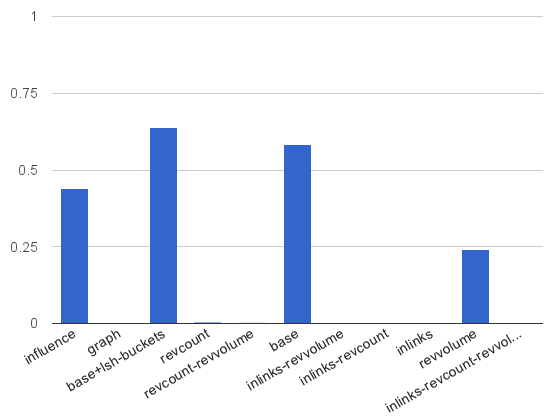
\includegraphics[width=0.9\textwidth,natwidth=555,natheight=419]{images/rand-mean.png}
  \caption{The score of the \emph{random selected} sets as given by the other
  submodular functions}
  \label{img:rand-mean}
\end{figure}

Looking at Figure~\ref{img:rand-mean} we see that methods that rely solely on
\emph{tf-idf} -- even if in more processed forms, such in the case of
\emph{document influence} give high scores to the randomly selected sets:
\begin{itemize}
  \item document influence \(\approx 0.44 (\pm 0.037)\);
  \item word coverage \(\approx 0.58 (\pm 0.025)\);
  \item word coverage + LSH buckets \(\approx 0.64 (\pm 0.021)\);
\end{itemize}
While all the sets have scores higher than random for all of these mentioned
functions, the high scores that random receives from these functions hints that
there do not represent a great measure for Wikipedia -- in other words, their
informativeness does not scale up to massive corpora.
Apart from these functions, also \emph{revisions volume} seems to be a less
informative measure as a lot of articles have a high volume of revisions.
The random sets receive the following score from the \emph{inlinks -- revision
volume} function: \(\approx 0.24 (\pm 0.025)\).

\subsection{Word coverage}

We present the \emph{functions scores} in Figure~\ref{img:wc} and the \emph{top
20} articles in Table~\ref{tab:wc}.

\begin{figure}
  \centering
  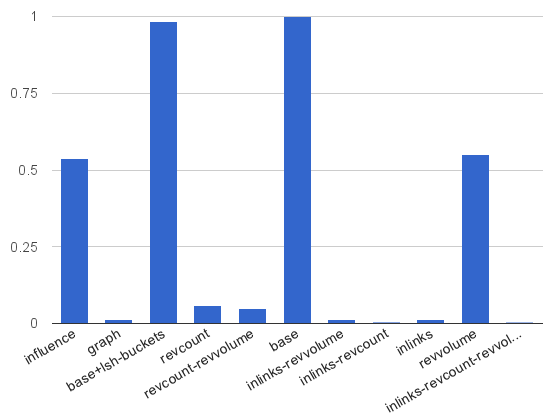
\includegraphics[width=0.9\textwidth,natwidth=555,natheight=419]{images/wc.png}
  \caption{The score of the \emph{word coverage} set as given by the other
  submodular functions}
  \label{img:wc}
\end{figure}

\begin{table}
    \begin{tabular}{lll}
    1  & History of Western civilization                  & 115   \\
    2  & Stephen Tompkinson                               & 78    \\
    3  & Timeline of United States inventions (1890–1945) & 381   \\
    4  & November 2013                                    & 102   \\
    5  & Education in the United States                   & 1098  \\
    6  & American Civil War bibliography                  & 320   \\
    7  & Races of the Mass Effect universe                & 42    \\
    8  & October 2011 in sports                           & 98    \\
    9  & Prince (musician)                                & 2458  \\
    10 & Stowe House                                      & 109   \\
    11 & Outline of science                               & 12    \\
    12 & 2000 New Year Honours                            & 77    \\
    13 & Seasons in Scottish football                     & 856   \\
    14 & Lists of state leaders by year                   & 2563  \\
    15 & The Idler (1758–1760)                            & 32    \\
    16 & National Football League                         & 22939 \\
    17 & Disasters of the Century                         & 8     \\
    18 & Sustainable Services                             & 1     \\
    19 & Australian of the Year                           & 232   \\
    20 & Largest organisms                                & 41    \\
    \end{tabular}
    \caption {Top 20 articles selected by the \emph{word coverage} function.}
    \label{tab:wc}
\end{table}

\subsection{Document influence}

We present the \emph{functions scores} in Figure~\ref{img:infl} and the
\emph{top 20} articles in Table~\ref{tab:infl}.

\begin{figure}
  \centering
  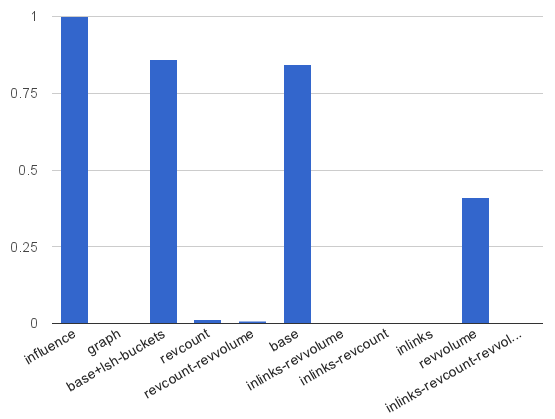
\includegraphics[width=0.9\textwidth,natwidth=555,natheight=419]{images/infl.png}
  \caption{The scores of the \emph{document influence} set as given by the
  other submodular functions}
  \label{img:infl}
\end{figure}

\begin{table}
    \begin{tabular}{lll}
    1  & History of virtual learning environments in the 1990s & 1   \\
    2  & The Idler (1758–1760)                                 & 32  \\
    3  & Economic history of China (1949–present)              & 0   \\
    4  & History of the Royal Australian Navy                  & 58  \\
    5  & Timeline of events in Hamilton, Ontario               & 257 \\
    6  & Technical features new to Windows Vista               & 23  \\
    7  & Outline of culture                                    & 34  \\
    8  & Seasons in Scottish football                          & 856 \\
    9  & Principles and Standards for School Mathematics       & 65  \\
    10 & \L\c{e}ka                                             & 0   \\
    11 & December 2003                                         & 88  \\
    12 & Coleman Station Historic District                     & 10  \\
    13 & Constitution of Fiji: Chapter 4                       & 195 \\
    14 & Jandek                                                & 128 \\
    15 & Partners in Flight                                    & 4   \\
    16 & Outline of software                                   & 3   \\
    17 & Dunorlan Park                                         & 102 \\
    18 & Bob and Carol Look for Treasure                       & 9   \\
    19 & Facility information model                            & 2   \\
    20 & Nationality Rooms                                     & 833 \\
    \end{tabular}
    \caption {Top 20 articles selected by the \emph{document influence}
    function.}
    \label{tab:infl}
\end{table}

As you can see from the graphs and tables for \emph{word coverage} and
\emph{document influence} the selected documents are not very informative of
any significant topic and scores of the functions are high only for the
functions we argued that are not very informative: \emph{tf-idf}-based and
\emph{revisions volume}-based functions.
In the following section we will show how the results can be improved
significantly (for Wikipedia).

\section{Graph coverage}

We present the \emph{functions scores} in Figure~\ref{img:graph} and the
\emph{top 20} articles in Table~\ref{tab:graph}.
\emph{Graph coverage} is a great improvement over previous methods, but has a
similar risk as the one associated with inlinks measures. For example, it picks
articles like \emph{Citation needed} that is clearly non-important, but it is
linked-to a lot.

\begin{figure}
  \centering
  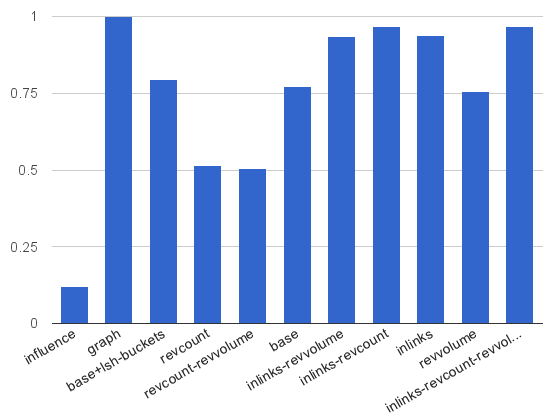
\includegraphics[width=0.9\textwidth,natwidth=555,natheight=419]{images/graph.png}
  \caption{The scores of the \emph{graph coverage} set as given by the other
  submodular functions}
  \label{img:graph}
\end{figure}

\begin{table}
    \begin{tabular}{lll}
    1  & Geographic coordinate system       & 759441 \\
    2  & Citation needed                    & 637433 \\
    3  & United States                      & 508227 \\
    4  & International Standard Book Number & 343361 \\
    5  & Biological classification          & 217533 \\
    6  & Music genre                        & 209333 \\
    7  & Internet Movie Database            & 183739 \\
    8  & Orphan                             & 171883 \\
    9  & Association football               & 96447  \\
    10 & United Kingdom                     & 181525 \\
    11 & Germany                            & 157768 \\
    12 & Canada                             & 149119 \\
    13 & Digital object identifier          & 109622 \\
    14 & England                            & 159822 \\
    15 & France                             & 179483 \\
    16 & India                              & 114069 \\
    17 & Public domain                      & 53717  \\
    18 & Japan                              & 113741 \\
    19 & Australia                          & 125675 \\
    20 & Given name                         & 27087  \\
    \end{tabular}
    \caption {Top 20 articles selected by the \emph{graph coverage} function.}
    \label{tab:graph}
\end{table}

\section{\ac{LSH} buckets and word coverage}

We present the \emph{functions scores} in Figure~\ref{img:wc+lsh} and the
\emph{top 20} articles in Table~\ref{tab:wc+lsh}.
As we mentioned in Section~\vref{sec:combine}, finding proper weights to
linearly combined multiple submodular functions is hard and as such \emph{word
coverage + LSH buckets} performs similarly to using just \emph{word coverage}.

\begin{figure}
  \centering
  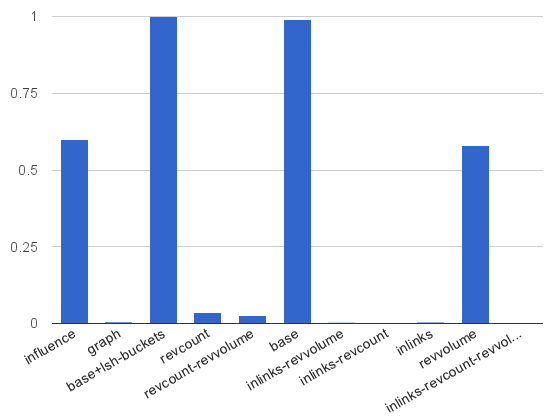
\includegraphics[width=0.9\textwidth,natwidth=555,natheight=419]{images/wc+lsh.png}
  \caption{The scores of the set selected by \emph{\ac{LSH} buckets} linearly
  combined with \emph{word coverage} as given by the other submodular
  functions}
  \label{img:wc+lsh}
\end{figure}

\begin{table}
    \begin{tabular}{lll}
    1  & History of Western civilization                              & 115  \\
    2  & Stephen Tompkinson                                           & 78   \\
    3  & Timeline of United States inventions (1890–1945)             & 381  \\
    4  & November 2003                                                & 102  \\
    5  & Education in the United States                               & 1098 \\
    6  & 2000 New Year Honours                                        & 77   \\
    7  & Races of the Mass Effect universe                            & 42   \\
    8  & November 2006 in sports                                      & 101  \\
    9  & Timeline of musical events                                   & 69   \\
    10 & The Idler (1758–1760)                                        & 32   \\
    11 & Systems engineering                                          & 874  \\
    12 & Long Beach, California                                       & 4273 \\
    13 & Seasons in Scottish football                                 & 856  \\
    14 & Asimov's Biographical Encyclopedia of Science and Technology & 0    \\
    15 & Tears for Fears                                              & 577  \\
    16 & Disasters of the Century                                     & 8    \\
    17 & The False Prince and the True                                & 4    \\
    18 & Economic history of China (1949–present)                     & 0    \\
    19 & 2012 in film                                                 & 736  \\
    20 & Independence National Historical Park                        & 359  \\
    \end{tabular}
    \caption {Top 20 articles selected by the \emph{LSH buckets} function.}
    \label{tab:wc+lsh}
\end{table}

\section{Beyond word coverage}

EXPLAIN \todo{Explain all results!}
CAPTIONS \todo{Change figure captions to meet the names of the functions}

We present the \emph{tf-idf \(\cdot\) number-of-revisions} in
Figure~\ref{img:rc} and the \emph{top 20} articles in Table~\ref{tab:rc}.
\begin{figure}
  \centering
  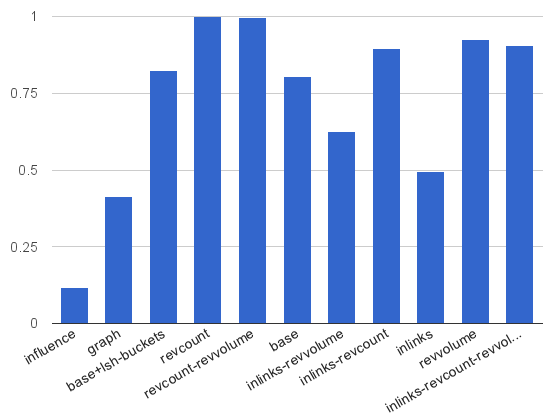
\includegraphics[width=0.9\textwidth,natwidth=555,natheight=419]{images/rc.png}
  \caption{The scores of the \emph{tf-idf -- revisions count} set as given by
  the other submodular functions}
  \label{img:rc}
\end{figure}
\begin{table}
    \begin{tabular}{lll}
    1  & George W. Bush      & 11525  \\
    2  & United States       & 508227 \\
    3  & Jesus               & 7065   \\
    4  & Adolf Hitler        & 7148   \\
    5  & Wii                 & 3860   \\
    6  & Michael Jackson     & 6661   \\
    7  & World War II        & 104037 \\
    8  & Hurricane Katrina   & 3875   \\
    9  & RuneScape           & 475    \\
    10 & United Kingdom      & 181525 \\
    11 & 2006 Lebanon War    & 793    \\
    12 & Britney Spears      & 3584   \\
    13 & The Beatles         & 10395  \\
    14 & 2007                & 723    \\
    15 & New York City       & 69267  \\
    16 & India               & 114069 \\
    17 & Islam               & 17455  \\
    18 & Global warming      & 3832   \\
    19 & PlayStation 3       & 3696   \\
    20 & 2006 FIFA World Cup & 3072   \\
    \end{tabular}
    \caption {Top 20 articles selected by the \emph{tf-idf -- revisions count}
function.}
    \label{tab:rc}
\end{table}

We present the \emph{tf-idf \(\cdot\) number-of-revisions \(\cdot\)
revisions-volume} in Figure~\ref{img:rc-rv} and the \emph{top 20} articles in
Table~\ref{tab:rc-rv}.
\begin{figure}
  \centering
  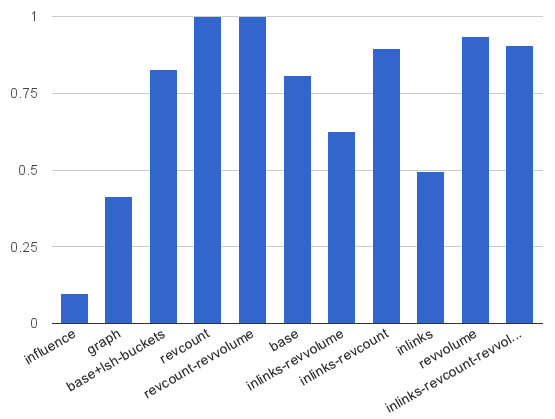
\includegraphics[width=0.9\textwidth,natwidth=555,natheight=419]{images/rc-rv.png}
  \caption{The scores of the \emph{tf-idf -- revisions count -- revisions
  volume} set as given by the other submodular functions}
  \label{img:rc-rv}
\end{figure}
\begin{table}
    \begin{tabular}{lll}
    1  & George W. Bush    & 11525  \\
    2  & United States     & 508227 \\
    3  & Jesus             & 7065   \\
    4  & Adolf Hitler      & 7148   \\
    5  & Michael Jackson   & 6661   \\
    6  & World War II      & 104037 \\
    7  & Wii               & 3860   \\
    8  & Hurricane Katrina & 3875   \\
    9  & RuneScape         & 475    \\
    10 & United Kingdom    & 181525 \\
    11 & Britney Spears    & 3584   \\
    12 & The Beatles       & 10395  \\
    13 & 2006 Lebanon War  & 793    \\
    14 & New York City     & 69267  \\
    15 & Islam             & 17455  \\
    16 & India             & 114069 \\
    17 & 2007              & 723    \\
    18 & PlayStation 3     & 3696   \\
    19 & Global warming    & 3832   \\
    20 & Christianity      & 17145  \\
    \end{tabular}
    \caption {Top 20 articles selected by the \emph{tf-idf -- revisions count
-- revisions volume} function.}
    \label{tab:rc-rv}
\end{table}

We present the \emph{tf-idf \(\cdot\) number-of-inlinks \(\cdot\)
revisions-volume} in Figure~\ref{img:inl-rv} and the \emph{top 20} articles in
Table~\ref{tab:inl-rv}.
\begin{figure}
  \centering
  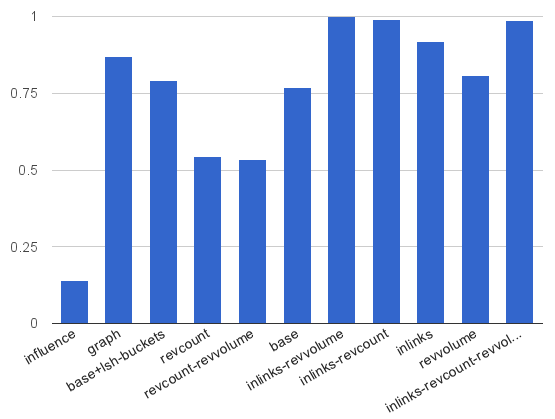
\includegraphics[width=0.9\textwidth,natwidth=555,natheight=419]{images/inl-rv.png}
  \caption{The scores of the \emph{tf-idf -- inlinks count -- revisions volume}
  set as given by the other submodular functions}
  \label{img:inl-rv}
\end{figure}

\begin{table}
    \begin{tabular}{lll}
    1  & United States                      & 508227 \\
    2  & Geographic coordinate system       & 759441 \\
    3  & France                             & 179483 \\
    4  & United Kingdom                     & 181525 \\
    5  & Time zone                          & 225085 \\
    6  & England                            & 159822 \\
    7  & International Standard Book Number & 343361 \\
    8  & Germany                            & 157768 \\
    9  & Internet Movie Database            & 183739 \\
    10 & Music genre                        & 209333 \\
    11 & Record label                       & 195384 \\
    12 & Poland                             & 108573 \\
    13 & Canada                             & 149119 \\
    14 & India                              & 114069 \\
    15 & Australia                          & 125675 \\
    16 & World War II                       & 104037 \\
    17 & Italy                              & 115868 \\
    18 & Daylight saving time               & 139888 \\
    19 & Animal                             & 133644 \\
    20 & Association football               & 96447  \\
    \end{tabular}
    \caption {Top 20 articles selected by the \emph{tf-idf -- inlinks count --
revisions volume} function.}
    \label{tab:inl-rv}
\end{table}

We present the \emph{tf-idf \(\cdot\) number-of-inlinks \(\cdot\)
number-of-revisions} in Figure~\ref{img:inl-rc} and the \emph{top 20} articles
in Table~\ref{tab:inl-rc}.
\begin{figure}
  \centering
  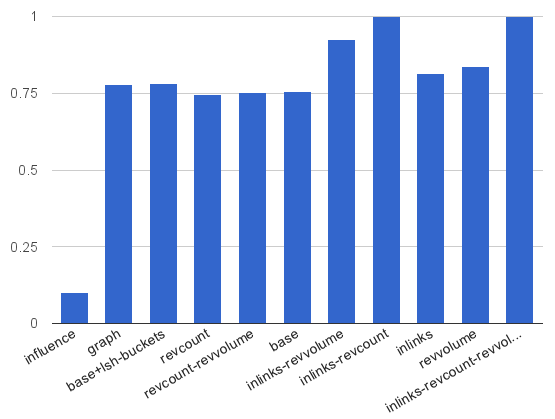
\includegraphics[width=0.9\textwidth,natwidth=555,natheight=419]{images/inl-rc.png}
  \caption{The scores of the \emph{tf-idf -- inlinks count -- revisions count}
  set as given by the other submodular functions}
  \label{img:inl-rc}
\end{figure}

\begin{table}
    \begin{tabular}{lll}
    1  & United States        & 508227 \\
    2  & United Kingdom       & 181525 \\
    3  & World War II         & 104037 \\
    4  & France               & 179483 \\
    5  & Germany              & 157768 \\
    6  & India                & 114069 \\
    7  & England              & 159822 \\
    8  & Canada               & 149119 \\
    9  & Japan                & 113741 \\
    10 & New York City        & 69267  \\
    11 & Australia            & 125675 \\
    12 & Italy                & 115868 \\
    13 & Association football & 96447  \\
    14 & Russia               & 84692  \\
    15 & George W. Bush       & 11525  \\
    16 & London               & 85152  \\
    17 & Poland               & 108573 \\
    18 & Spain                & 90482  \\
    19 & World War I          & 47384  \\
    20 & Brazil               & 73972  \\
    \end{tabular}
    \caption {Top 20 articles selected by the \emph{tf-idf -- inlinks count --
revisions count} function.}
  \label{tab:inl-rc}
\end{table}

We present the \emph{tf-idf \(\cdot\) number-of-inlinks} in
Figure~\ref{img:inl} and the \emph{top 20} articles in Table~\ref{tab:inl}.
\begin{figure}
  \centering
  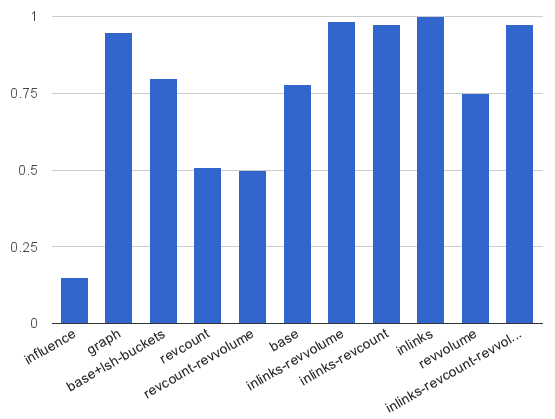
\includegraphics[width=0.9\textwidth,natwidth=555,natheight=419]{images/inl.png}
  \caption{The scores of the \emph{tf-idf -- inlinks count} set as given by the
  other submodular functions}
  \label{img:inl}
\end{figure}

\begin{table}
    \begin{tabular}{lll}
    1  & United States                      & 508227 \\
    2  & Geographic coordinate system       & 759441 \\
    3  & France                             & 179483 \\
    4  & Citation needed                    & 637433 \\
    5  & International Standard Book Number & 343361 \\
    6  & United Kingdom                     & 181525 \\
    7  & Time zone                          & 225085 \\
    8  & Biological classification          & 217533 \\
    9  & Record label                       & 195384 \\
    10 & England                            & 159822 \\
    11 & Internet Movie Database            & 183739 \\
    12 & Music genre                        & 209333 \\
    13 & Germany                            & 157768 \\
    14 & Poland                             & 108573 \\
    15 & Orphan                             & 171883 \\
    16 & Daylight saving time               & 139888 \\
    17 & India                              & 114069 \\
    18 & Canada                             & 149119 \\
    19 & Record producer                    & 119573 \\
    20 & Italy                              & 115868 \\
    \end{tabular}
    \caption {Top 20 articles selected by the \emph{tf-idf -- inlinks count}
function.}
    \label{tab:inl}
\end{table}

We present the \emph{tf-idf \(\cdot\) revisions-volume} in Figure~\ref{img:rv}
and the \emph{top 20} articles in Table~\ref{tab:rv}.
\begin{figure}
  \centering
  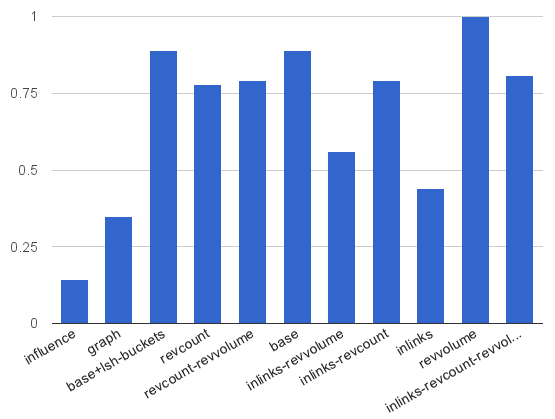
\includegraphics[width=0.9\textwidth,natwidth=555,natheight=419]{images/rv.png}
  \caption{The scores of the \emph{tf-idf -- revisions volume} set as given by
  the other submodular functions}
  \label{img:rv}
\end{figure}

\begin{table}
    \begin{tabular}{lll}
    1  & George W. Bush           & 11525  \\
    2  & World War I              & 47384  \\
    3  & United States            & 508227 \\
    4  & Michael Jackson          & 6661   \\
    5  & England                  & 159822 \\
    6  & Jesus                    & 7065   \\
    7  & Jack Thompson (activist) & 35     \\
    8  & Internet                 & 11878  \\
    9  & Baseball                 & 22619  \\
    10 & Gray wolf                & 916    \\
    11 & The Beatles              & 10395  \\
    12 & 2007                     & 723    \\
    13 & Water                    & 8390   \\
    14 & France                   & 179483 \\
    15 & Hurricane Katrina        & 3875   \\
    16 & Punk rock                & 12159  \\
    17 & Microsoft                & 9842   \\
    18 & Pope John Paul II        & 5314   \\
    19 & Association football     & 96447  \\
    20 & Evolution                & 3867   \\
    \end{tabular}
    \caption {Top 20 articles selected by the \emph{tf-idf -- revisions volume}
function.}
    \label{tab:rv}
\end{table}

We present the \emph{tf-idf \(\cdot\) number-of-inlinks \(\cdot\)
number-of-revisions\(\cdot\) revisions-volume} in Figure~\ref{img:inl-rc-rv}
and the \emph{top 20} articles in Table~\ref{tab:inl-rc-rv}.
\begin{figure}
  \centering
  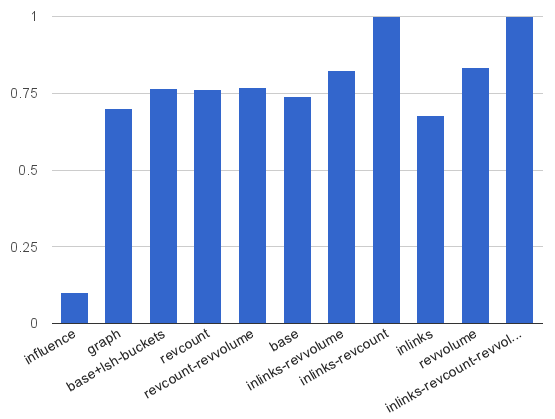
\includegraphics[width=0.9\textwidth,natwidth=555,natheight=419]{images/inl-rc-rv.png}
  \caption{The scores of the \emph{tf-idf -- inlinks count -- revisions count
  -- revisions volume} set as given by the other submodular functions}
  \label{img:inl-rc-rv}
\end{figure}

\begin{table}
    \begin{tabular}{lll}
    1  & United States        & 508227 \\
    2  & United Kingdom       & 181525 \\
    3  & World War II         & 104037 \\
    4  & France               & 179483 \\
    5  & Germany              & 157768 \\
    6  & England              & 159822 \\
    7  & Canada               & 149119 \\
    8  & India                & 114069 \\
    9  & Japan                & 113741 \\
    10 & New York City        & 69267  \\
    11 & Australia            & 125675 \\
    12 & Italy                & 115868 \\
    13 & George W. Bush       & 11525  \\
    14 & Association football & 96447  \\
    15 & Russia               & 84692  \\
    16 & World War I          & 47384  \\
    17 & London               & 85152  \\
    18 & Poland               & 108573 \\
    19 & Spain                & 90482  \\
    20 & Brazil               & 73972  \\
    \end{tabular}
    \caption {Top 20 articles selected by the \emph{tf-idf -- inlinks count --
revisions count -- revisions volume} function.}
  \label{tab:inl-rc-rv}
\end{table}

\section{Running time}

Dummy text. \todo{Add running times}

